\chapter{实验分析}
\label{chapter:evaluation}
本章将对前文中设计并实现的高性能NFV实现平台进行试验分析及性能测试。我们首先对使用的实验平台和实验环境进行详细的介绍,然后针对每一种具体的实验方案进行展开说明,包括进行试验数据归纳和分析。最后,对实验的总体效果和系统的实际收益进行总结。

\section{实验平台和测试环境}
实验中主要使用了一台浪潮英信大通量标准通用服务器,将其作为虚拟化平台,支持虚拟机的创建、运行和销毁。该测试服务器配置有4颗8核2.13GHz的Intel Xeon至强 E7-4830 CPU,以及128G大小的DDR3内存,并且配有1T容量的标准容量SATA磁盘作为外部储存设备。为了真实考察所设计的系统在实际生产环境中所能达到的实际优化效果,实验测试的进行均在真实的实验室网络环境中,而运行的NFV应用为真实的IP多媒体子系统 ClearWater,可以运行真实的语音视频通话业务。在软件配置方面,宿主机上安装的是7.3版本的CentOS Linux操作系统,使用系统自带的KVM作为虚拟化监视器,而且所有的虚拟机均安装的14.04版本的Ubuntu操作系统。除了NFV服务自身的软件,系统中没有安装其他任何多余的软件,以排除不必要的软件因素的干扰并且将系统运行时的额外性能损失降到最低。服务器的具体配置参数如表 \ref{tab:configure} 所示。

从测试工具及实验手段的角度来说,本章中主要使用了Clearwater平台自带的压力测试工具和主流的性能测试和评估工具如Ping、iPerf\footnote{https://iperf.fr/}、Apache\footnote{http://httpd.apache.org/}等,从具体的业务性能到通用的性能测试两个层次进行了深入、翔实的实验。从实验对象上来说,主要的实验集中在对系统网络性能的测试和评估上。从实验目的上来说,本章的实验设计主要从具体业务和网络性能两方面出发,分别对本文所提出的系统进行了测试。实验内容包括:1.Clearwater压力测试工具的性能测试对比。2.Ping、iPerf、Apache工具的基础性能测试对比。

\begin{table}[htb]
	\centering
	\bicaption[tab:configure]{实验平台配置参数表}{实验平台配置参数表}{Table}{Table of Testing Environment Configuration}
	\begin{tabular}{ | l | p{6cm} |}\hline
		\textbf{项目} &							 \textbf{配置}  				\\ 	\hline
		服务器        &					 浪潮 NF8560M2, 4节点NUMA架构\\ \hline
		处理器 	   &  Intel Xeon CPU E7-4830,2.13GHz x 4  \\ \hline
		缓存    & 24M L3, 256K L2,  64K L1 \\ \hline
		内存 			&  每个节点32GB DDR3,  共128G   \\   \hline
		硬盘     & 				1 TB SATA disk \\ \hline
		操作系统    & Hypervisor: CentOS Linux 7.3,  Virtual Machine Ubuntu 14.04 \\ \hline
	\end{tabular}
\end{table}

\begin{figure}[!htp]
	\centering
	\subfigure[离散分布]{
		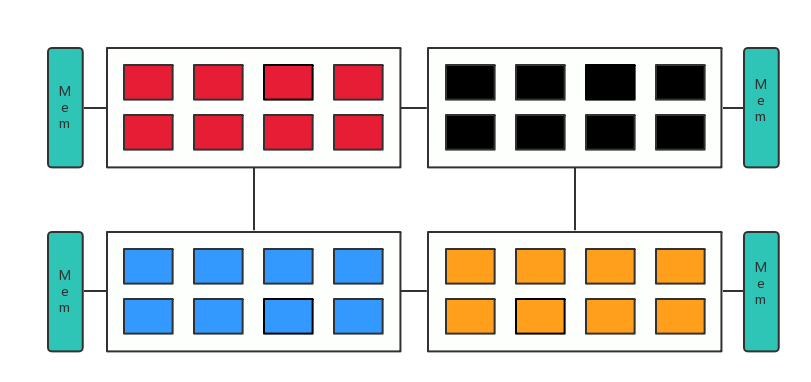
\includegraphics[width=0.8\textwidth]{distribution/Scattering.png}
	}
	\subfigure[聚合分布]{
		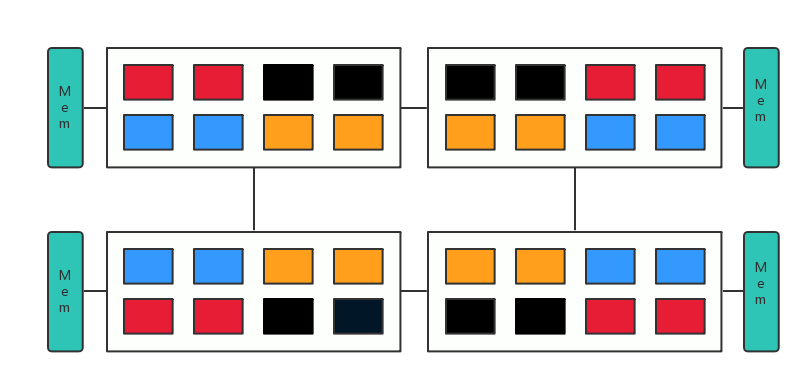
\includegraphics[width=0.8\textwidth]{distribution/Uniform.png}
	}
	\subfigure[随机分布]{
		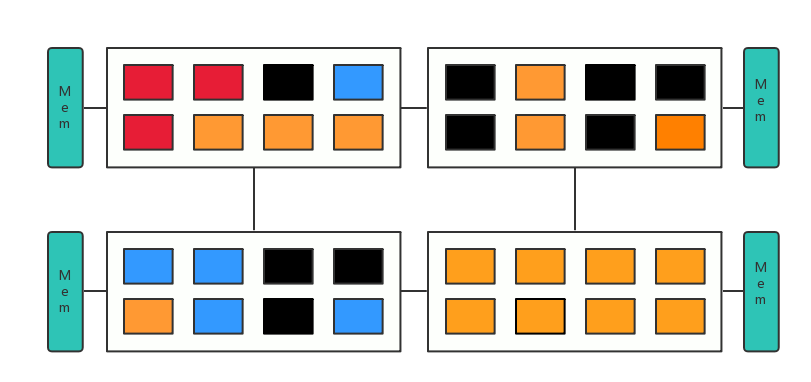
\includegraphics[width=0.8\textwidth]{distribution/Random.png}
	}
	\bicaption[fig:resource]{实例分布示意图}{实例分布示意图}{Fig}{Resource Distribution}
\end{figure}
除了使用以上所述的测试工具,我们充分考虑了在实际环境下各种网络功能实例在多核物理机上的分布情况,故我们列举三种可能的实例分布方式如图 \ref{fig:resource} 所示,分别为离散分布、随机分布和聚合分布。图中以不同的色块来代表不同的网络功能,以实例所绑定的物理CPU来代表某个实例的物理资源分配情况。可以看出,在离散分布的情形下,相同的虚拟网络功能实例聚集在同一个处理器节点中,在这样的资源分布下,所有虚拟机实例间具有相近的物理资源亲和度。在聚合分布下,每个处理器节点上都被均匀地绑定了实现网络服务链的所有功能实例。而在随机分布的情形下,所有的网络功能实例以随机的方式绑定在所有的物理CPU上。我们后续的所有测试将覆盖这三种资源分布的前提,以检验我们系统的适用性以及在不同物理资源环境中的可行性。


\section{Clearwater压力测试实验}
我们以按照分布式的方式在配置如 \ref{tab:configure} 所示的大通量标准服务器中部署了Clearwater所需的所有功能节点,以KVM作为Hypervisor,所有虚拟机均配置了单个虚拟核、1G的运行内存和10G的磁盘容量,并利用Virtio的网络虚拟化方式提供虚拟网卡。测试负载方面,我们使用了Clearwater平台所提供的测试工具集,选择了其中的标准语音通信业务中用户注册-解注册业务\textit{reg-dereg}作为我们的测试负载。一次\textit{reg-dereg}服务由三个请求组成,分别为:注册请求、认证请求和注销请求。其中任意一个请求一旦超过了最大返回等待时间(10s),则该次请求失败。我们每次实验指定运行300s,运行10次后去平均值作为最终结果。测试工具可以指定不同的初始请求速率来测试不同负载强度下的平均请求响应延迟。我们使用从发起注册请求到最后一个请求的200回执为止的平均时间作为衡量延迟的具体参数,单位为毫秒。最后我们以平均的延迟时间和请求的成功率来作为性能比较的依据。

\begin{figure}[htp]
	\centering
	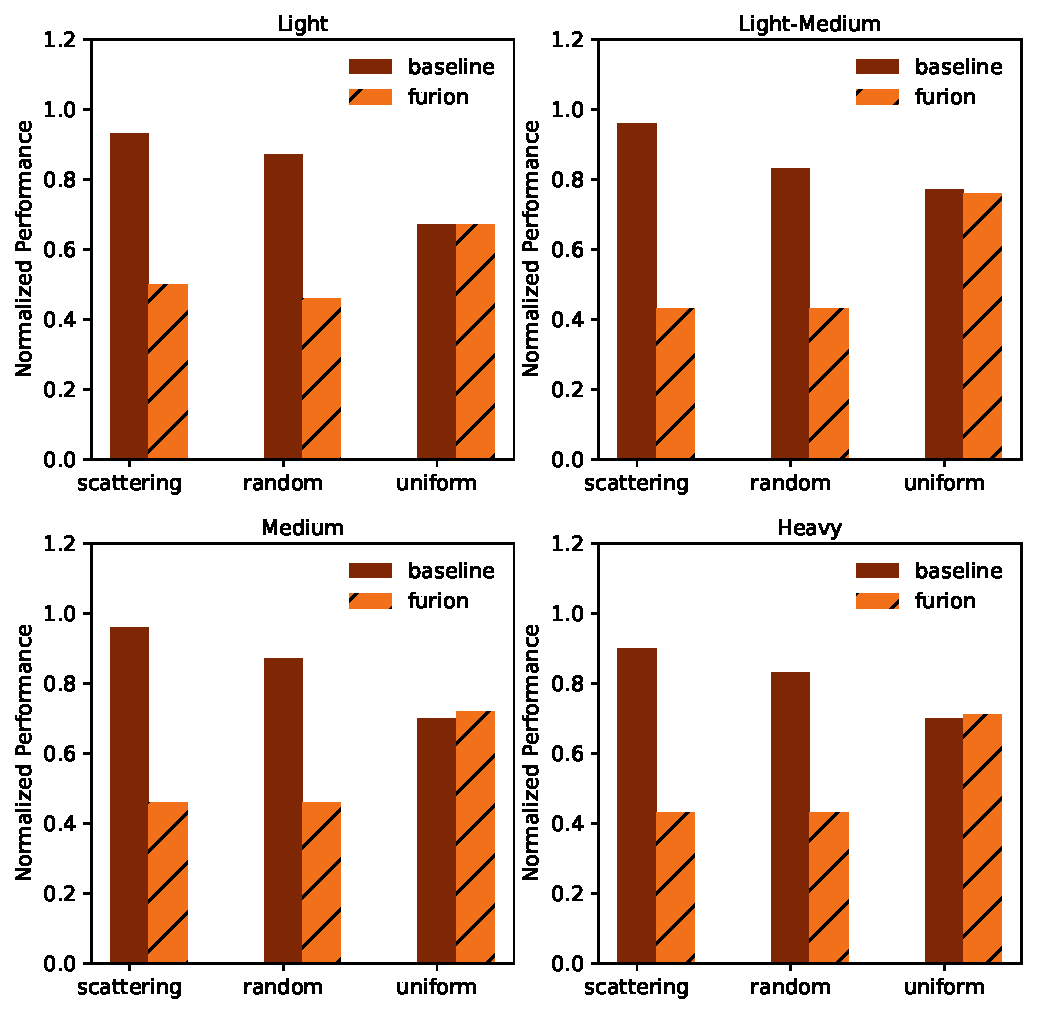
\includegraphics[width=0.8\textwidth]{clearwater.pdf}
	\bicaption[exp:clearwater]{ClearWater压力测试结果图}{ClearWater压力测试结果图}{Fig}{Clearwater Performance Test}
\end{figure}

压力测试实验结果如图 \ref{exp:clearwater} 所示,我们测试了在light (50),light-medium(100),medium(500),heavy(1000) 四种请求速率下默认系统与我们所实现的系统在性能上的差异,在这四种负载下分别测试了三种不同分布下的性能结果作为对照组。深色的柱状条代表默认的系统的测试结果,浅色的柱状条代表在我们系统优化过后结果。为了方便比较,我们对数据进行了归一化处理,这样能够比较直观的体现出优化前后的性能对比。根据图 \ref{exp:clearwater} ,我们可以看出在四种不同大小的负载下,我们的系统在离散分布和随机分布中都取得了较好的优化效果,服务的延迟平均有接近40\%的下降,而在聚合分布的情况下,服务在优化前后并没有表现出较大的性能差别。进一步的我们对比三种分布下的基准和优化的平均性能,不难发现,聚合分布的平均性能最高随机分布次之而离散分布最差,而经过我们的优化之后,离散和随机的分布下得平均延迟均低于聚合分布。这样的测试结果基本上是符合我们对测试结果的预期的。首先,针对离散和随机分布,在默认条件下Clearwater系统会随机的选取实例进行组链,完全没有考虑资源间的亲和性,故在这种情况下所产生服务链就会有较大的服务延迟,而且由于资源分布的离散程度,不同资源之间的亲和度具有不同级别的差异。对比聚合分布下,所有的功能实例与其他的功能实例的具有相同的亲和度,所平均性能比较稳定,也不存在可以优化的提升空间,故默认系统和优化后的系统并没有显示出性能差异。

综合来看,我们的优化系统在大部分情况下确实能够提升实际NFV服务的性能。

\section{基础网络性能对比实验}
根据系统在运行所选取的具体虚拟机所组成的服务链,我们除了使用Clearwater自带的压力测试工具测量IMS业务性能之外,也使用了一些基础的测试工具对类似的NFV业务进行和仿真测试,用来验证我们系统的通用型和优化的有效性。为了模拟实际NFV服务的SFC,我们将系统所选择的服务链实例挑选出来,分别用Ping,iPerf和Apache Bench来进行端对端的性能测试,并将其结果累计算作服务链的性能结果进行比较和验证优化系统的有效性。同样的,我们测试了在三种不同实例分布的下的SFC映射结果。

\subsection{Ping实验}
在本小节中,我们使用了轻量级的网络命令Ping来测试系统的累计网络延迟性能。Ping是一个非常轻量级的网络命令,其运行过程中的所引起的CPU和内存额外开销可以忽略不计,因而在网络测试中Ping命令经常被用来测试网络的延迟大小,测试的结果基本与真实网络链路上产生的延迟相等。在小节的实验中,所有的虚拟机依然采用单个虚拟核、1G运行内存和10G磁盘的配置,测试的虚拟机使用Ubuntu 14.04 Server版本的系统。为了获取服务链累计的延迟信息,我们设置了链路上每一个上游节点都同时向自己相邻的下游节点进行Ping请求,并将每台客户端的测试结果输出并统计。实验所使用的发包时间间隔为0.5秒,测试时间长度为1分钟。
\begin{figure}[!htp]
	\centering
	\subfigure[离散分布下Ping测试结果]{
		\label{exp:ping_scattering}
		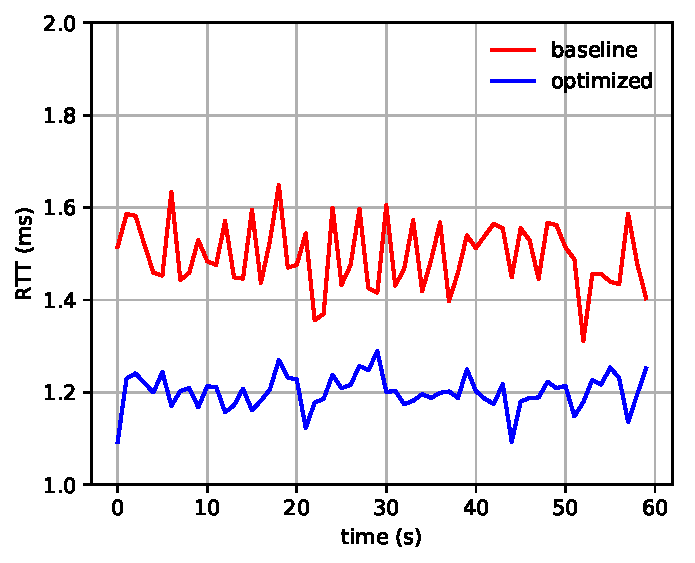
\includegraphics[width=0.75\textwidth]{ping/ping_scattering.pdf}
	}
	\subfigure[聚合分布下Ping测试结果]{
	\label{exp:ping_uniform}
	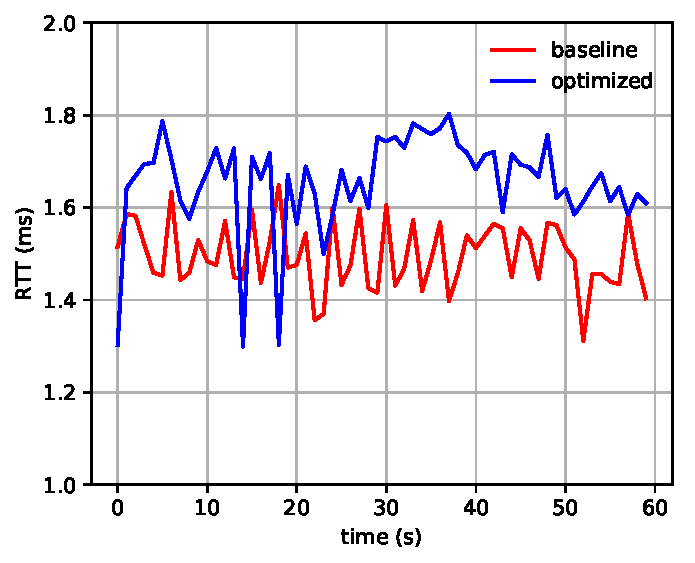
\includegraphics[width=0.75\textwidth]{ping/ping_uniform.pdf}
	}
	\bicaption[exp:ping]{Ping测试结果图}{Ping测试结果图}{Fig}{Ping Test Result}
	
\end{figure}
\begin{figure}
	\addtocounter{subfigure}{2}
	\ContinuedFloat
	\centering
	\subfigure[随机分布下Ping测试结果]{
	\label{exp:ping_random}
	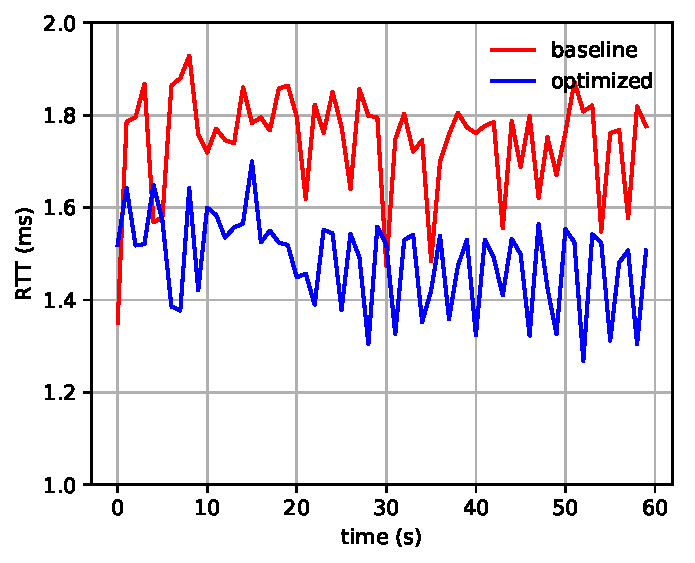
\includegraphics[width=0.75\textwidth]{ping/ping_random.pdf}
	}

	\bicaption[exp:ping]{Ping测试结果图 (续)}{Ping测试结果图 (续)}{Fig}{Ping Test Result (Con't)}
\end{figure}

如图 \ref{exp:ping} 所示,红色的折线代表默认的服务链映射策略所选的实例组合所产生的累计延迟,蓝色的折线代表优化系统所选择实例所产生的累计延迟。在统计过程中我们发现,虽然端到端的Ping测试结果差异比较小,但是当服务链的所有节点的延迟累计起来后,延迟的下降就相对明显了。在离散和随机分布中,如图 \ref{exp:ping_scattering} 和图 \ref{exp:ping_random} 所示,我们观测到了对于每条服务链,都有接近0.2ms的延迟下降,下降的比例接近15\%。而在聚合分布下,优化前后的性能差异也并不明显。对比三种分布下的延迟数据,我们有可以看出,在离散分布的设定下,服务链可以达到最低的累计延迟,相比于最高的随机分布,有了接近30\%的延迟下降。


\subsection{iPerf实验}
本节中,我们使用iPerf工具来测试系统的网络带宽性能。iPerf是一套可以动态测量基于IP网络的最大执行带宽的测试工具集。它支持调整执行时间、协议和缓冲区大小来进行性能调优。本小节的实验中我们使用的是更加轻量级的iPerf3来进行测试,测试虚拟机的而配置与Ping实验中的相同。iPerf测试需要手动配置客户端和服务端,因此我们在所有运行的虚拟机中都配置iPerf服务监听端口,当获取实际链路组合后,以链路上每个前置节点作为客户端向相邻的后置节点发送数据,统计链路上的累计带宽。单次实验的执行时间为30秒,分别使用了数据包大小为1K、4K、16K的测试负载来针对三种不同的实例分布进行了测试,每组实现均执行10次取平均值作为最后的输出结果。
\begin{figure}[!htp]
	\centering
	\subfigure[离散分布下的iPerf测试结果]{
		\label{exp:iperf_scattering}
		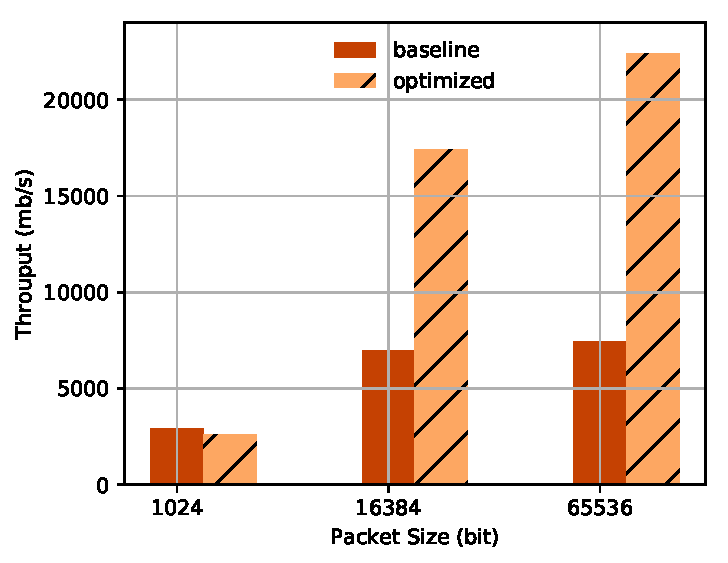
\includegraphics[width=0.75\textwidth]{iperf/iperf_scatter.pdf}
	}
	\subfigure[聚合分布下的iPerf测试结果]{
		\label{exp:iperf_uniform}
		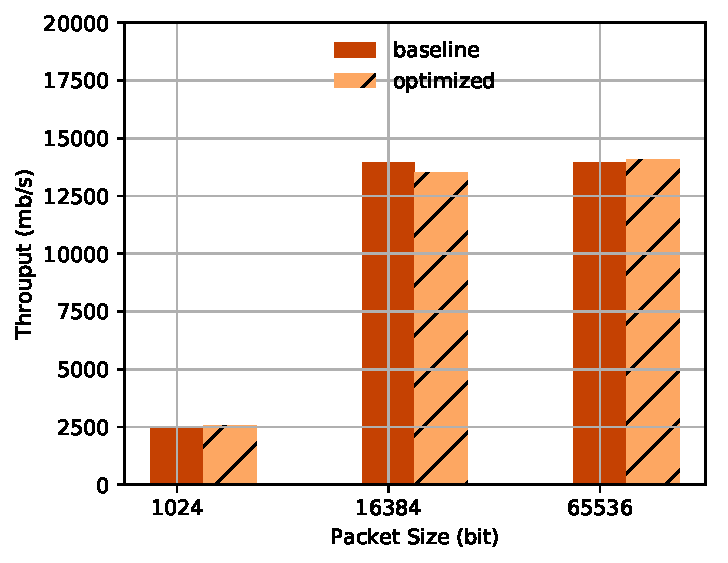
\includegraphics[width=0.75\textwidth]{iperf/iperf_uniform.pdf}
	}
	\bicaption[exp:iPerf]{iPerf测试结果图}{iPerf测试结果图}{Fig}{iPerf Test Result}
\end{figure}
\begin{figure}
	\addtocounter{subfigure}{2}
	\ContinuedFloat
	\centering
	\subfigure[随机分布下的iPerf测试结果]{
	\label{exp:iperf_random}
	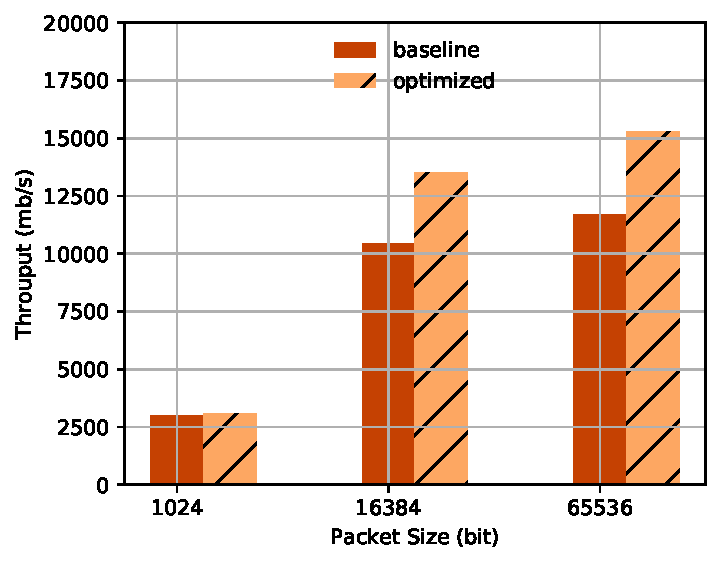
\includegraphics[width=0.75\textwidth]{iperf/iperf_random.pdf}
	}
	\bicaption[exp:iPerf]{iPerf测试结果图 (续)}{iPerf测试结果图 (续)}{Fig}{iPerf Test Result (Con't)}
\end{figure}

如图 \ref{exp:iPerf} 所示,深色的柱状条代表默认的随机的选取策略所选取的服务链实例组合在iPerf测试场景下的性能测试结果,浅色斜杠条纹柱状条则代表本文优化策略所选取的服务链组合的测试性能测试结果。通过统计我们可以明显发现,在离散分布和随机分布的情况下,服务链的累计带宽有了明显的提升,特别是如图 \ref{exp:iperf_scattering} 所示在离散分布的16K数据包的测试对照组中,优化后的服务链相比于随机选择的组合,带宽有了接近3倍的提升。但是在1K数据包的测试对照组下,我们发现优化前后的性能变化并不大。通过监测实验时的实时CPU利用率,我们发现当发送1K数据包时,所有的运行实例的CPU接近满负载。结合我们已知的网络和操作系统知识来分析,在小包的情况下,限制网络带宽的瓶颈在于频繁的数据包处理,数据包数量越多,则CPU处理所需要的开销越高,故在小包情况下,服务链上的资源亲和度并没有对性能有主导影响。而随着数据包大小的提升,我们可以发现此时各实例之间的资源亲和度的影响逐渐增大,当数据包大小为16K时,更是出现了接近3倍的性能差距。这样的实验结果更是可以证明我们系统相比于随机策略的优越性。在分配相同的物理资源的条件下,我们可以获得最大接近3倍的网络带宽提升。

\subsection{Apache实验}
本节中,我们使用ApacheBench来测试在模拟真实业务下NFV服务链的标准性能。ApacheBench是一款用于测量HTTP Web服务器性能的测试工具,最初作为Apache HTTP Server的测试工具,后来被扩展为可以用于测试任何Web服务器。众所周知,NFV的业务纷繁复杂,仅仅使用不同大小的数据从微观的角度去衡量服务链的性能在实际应用场景下没有说服力,所以我们使用真实的Web服务来测试在真实网络应用场景下的实际性能。在实际应用场景下,业务请求可能包括不同大小不同长度的数据包,因为在这样的测试场景下进行测试更具有实际意义。Apache Bench的测试原理是由客户单向目标服务器发起资源请求,可以通过命令来创建不同数量的并发访问线程,模拟多个访问者对同一个URL地址进行访问。测试工具会持续访问资源直到完成预先设置的访问总数,并输出每秒所完成的请求次数。我们仿照之前的测试设置,使用了相同的虚拟机配置,在不同映射策略下的虚拟机之间根据服务链数据流的先后关系,进行了累计请求统计,除了不同的实例分布场景,我们选择不同请求并发数来考察在不同数据压力负载下的的性能表现,预先设置的访问总数为10万次,每次测试重复10次取平均结果来作为衡量依据。
\begin{figure}[!htp]
	\centering
	\subfigure[离散分布下的Apache Bench测试结果]{
		\label{exp:ab_scattering}
		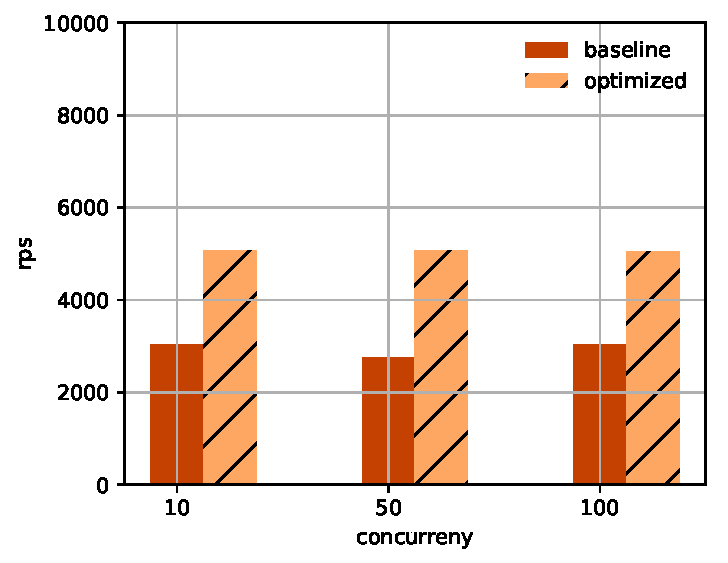
\includegraphics[width=0.75\textwidth]{ab/ab_scatter.pdf}
	}
	\subfigure[聚合分布下的Apache Bench测试结果]{
		\label{exp:ab_uniform}
		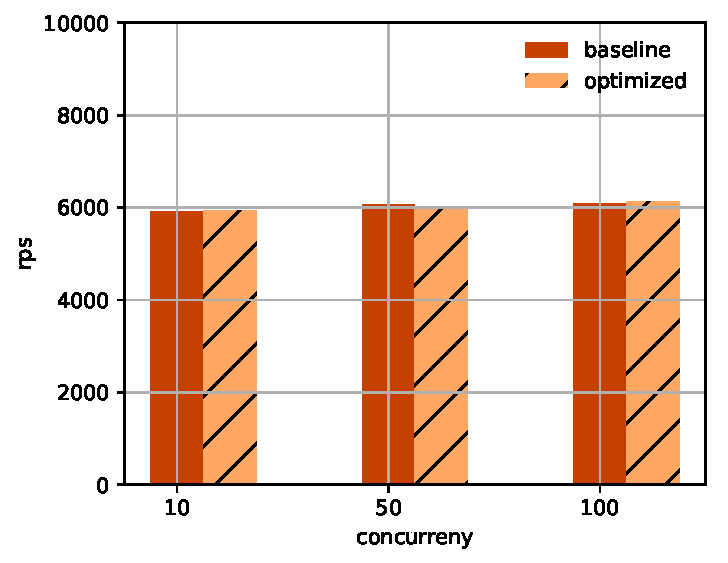
\includegraphics[width=0.75\textwidth]{ab/ab_uniform.pdf}
	}
	\bicaption[exp:ab]{Apache Bench测试结果图}{Apache Bench测试结果图(续)}{Fig}{Apache Bench Test Result}
\end{figure}
\begin{figure}
\addtocounter{subfigure}{2}
\ContinuedFloat
\centering
	\subfigure[随机分布下的Apache Bench测试结果]{
	\label{exp:ab_random}
	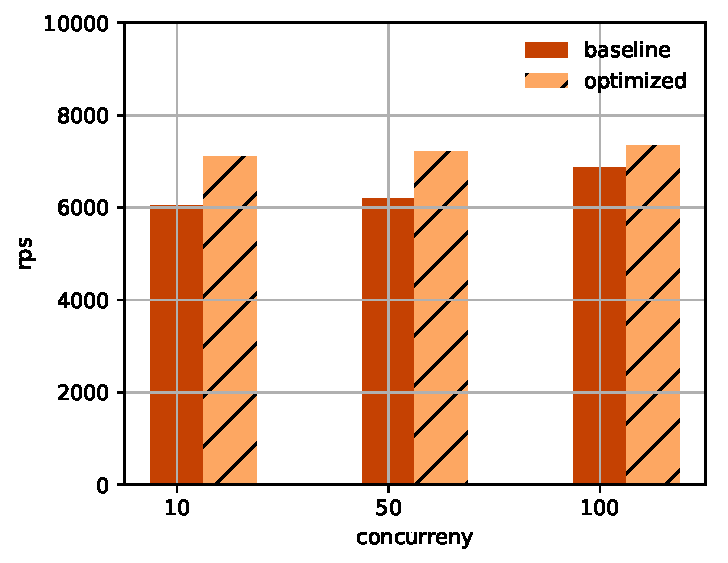
\includegraphics[width=0.75\textwidth]{ab/ab_random.pdf}
	}
\bicaption[exp:ab]{Apache Bench测试结果图 (续)}{Apache Bench测试结果图 (续)}{Fig}{Apache Bench Test Result (Con't)}
\end{figure}

Apache Bench的测试结果如图 \ref{exp:ab} 所示,深色的柱状条代表默认的随机选取策略的服务链在Apache Bench测试场景下的每秒的所能达到的累计请求完成数,浅色斜杠条纹柱代表在优化策略下测试组的测试结果。通过测试数据的整理我们可以发现,在线程数为10、50、100的并发请求下,优化后的系统在离散分布下由3000 rps左右提升到了5000 rps左右,在随机分布下由由6000 rps提升到了7500 rps左右。可以看出实际应用负载下,我们的系统对于性能的提升也是十分明显的。

\newpage
\section{本章小结}
本章主要介绍了基于底层感知的高性能NFV实现系统实验相关的部分内容。首先,本章介绍了实验所采用的软硬件平台,包括物理机的配置、虚拟化环境的和Clearwater平台的配置,引入了不同实例分布情况的分类说明。其实,我们对优化前后的系统进行了NFV应用的压力测试和基础网络性能测试的对比实验。压力测试用的是Clearwater提供的压力测试脚本工具,基础网络性能测试使用的工具包括Ping、iPerf、Apache Bench三种。压力测试所涵盖的性能测试主要包括请求的响应时间和成功率,基础网络测试所涵盖的性能点主要包括网络I/O的吞吐率、网络响应速率和网络的带宽。从实验数据的角度上证明了本文所提出的系统对NFV应用所带来的可观的性能提升,并且具有较好的适用性和扩展性。